\documentclass[10pt,a4paper]{article}
\usepackage{matlab-prettifier,amssymb,listings,titlesec, amsmath}
\usepackage[margin=2.0cm]{geometry}
\usepackage{multirow}
\usepackage{longtable}
\usepackage{graphicx}
\usepackage{setspace}

\titleformat*{\section}{\large\bfseries}

  \title{Anno accademico 2022-2023 \\ \vspace{20px} \textbf{Elaborato Calcolo Numerico}}

  \author{Autori: \textbf{Cavicchioli Michael}\\
  \texttt Matricole: \textbf{7051110}
  \and
  \textbf{Wu Jinkang}\\
  \textbf{7029446}
  \date{}}

\begin{document}

\maketitle

\newpage

\section{Verificare che:
  \[ -\frac{1}{4}f(x-h) -\frac{5}{6}f(x) + \frac{3}{2}f(x+h)
    -\frac{1}{2}f(x+2h) +\frac{1}{12}f(x+3h) = hf'(x) + O(h^5) \]}

\textbf{Soluzione:}
Come primo step siamo andati a calcolare il polinomio di Taylor, centrato in \textit{x},
per ogni membro presente nell'equazione.
\begin{align*}
  f(x-h) = f(x) - hf'(x) + \frac{h^2}{2}f''(x) - \frac{h^3}{6}f'''(x) + \frac{h^4}{24}f''''(x) + O(h^5) \\
  f(x+h) = f(x) + hf'(x) + \frac{h^2}{2}f''(x) + \frac{h^3}{6}f'''(x) + \frac{h^4}{24}f''''(x) + O(h^5) \\
  f(x+2h) = f(x) + 2hf'(x) + 2h^2f''(x) + \frac{4h^3}{3}f'''(x) + \frac{2h^4}{3}f''''(x) + O(h^5)       \\
  f(x+3h) = f(x) + 3hf'(x) + \frac{9h^2}{2}f''(x) + \frac{9h^3}{2}f'''(x) + \frac{27h^4}{8}f''''(x) + O(h^5)
\end{align*}
Successivamente, abbiamo sostituito i valori trovati nell'equazione di partenza:
\begin{align*}
  - \frac{1}{4}f(x-h)-\frac{5}{6}f(x)+\frac{3}{2}f(x+h)-\frac{1}{2}f(x+2h)+\frac{1}{12}f(x+3h) =                            \\
  - \frac{1}{4}f(x) + \frac{h}{4}f'(x) - \frac{h^2}{8}f''(x) + \frac{h^3}{24}f'''(x) - \frac{h^4}{96}f''''(x) +             \\
  - \frac{5}{6}f(x) +                                                                                                       \\
  + \frac{3}{2}f(x) + \frac{3h}{2}f'(x) + \frac{3h^2}{4}f''(x) + \frac{h^3}{4}f'''(x) + \frac{h^4}{16}f''''(x) +            \\
  - \frac{1}{2}f(x) - hf'(x) - h^2f''(x) - \frac{2h^3}{3}f'''(x) - \frac{h^4}{3}f''''(x) +                                  \\
  + \frac{1}{12}f(x) + \frac{h}{4}f'(x) + \frac{3h^2}{8}f''(x) + \frac{3h^3}{8}f'''(x) + \frac{9h^4}{32}f''''(x) + O(h^5) = \\
  + hf'(x) + O(h^5)
\end{align*}
Infine, abbiamo ugualiato il risultato trovato, con la parte destra dell'equazione
\[ hf'(x) + O(h^5) = hf'(x) + O(h^5) \]
dimostrando quanto richiesto.

\section{Matlab utilizza la doppia precisione IEEE. Stabilire, pertanto,
  il nesso tra la variabile eps e la precisione di macchina di questa aritmetica.}

E' noto che la precisione di macchina \textit{u}, nel caso di arrotondamento, si ottiene come: \textit{\[u =\frac{1}{2}b^{1-m}\]}
dove b corrisponde alla base scelta, mentre m e' il numero di cifre usate per la mantissa. Nello standard IEEE la base b corrisponde a 2,
mentre il numero usato per la mantissa e' pari a 52. Allora, la precisione di macchina sara':  \textit{\[u =\frac{1}{2}2^{1-52}=2^{-52}\]}
Questo valore e' il medesimo contenuto nella variabile \textbf{eps} di Matlab.
Infatti, la precisione di macchina e' definita come il massimo errore relativo dovuto alla rappresentazione in aritmetica finita di un numero reale.

\section{Spiegare il fenomeno della cancellazione numerica. Fare un esempio che la illustri, spiegandone i dettagli.}

La cancellazione numerica consiste nella perdita di cifre
significative, nel risultato derivante dalla somma di addendi
quasi opposti. Questo rispecchia il mal condizionamento di
questa operazione. Infatti, se X e Y sono i due numeri da sommare,
il numero di condizione si vede essere dato da:
\[
  \frac{|X| + |Y|}{|X + Y|}
\] che non e' limitato superiormente se: $$ X \approx -Y $$

\section{Scrivere una function Matlab, radice\textit{(x)} che, avendo in ingresso un numero x non negativo,
calcoli $ \sqrt[6]{x} $ utilizzando solo operazioni algebriche elementari, con la massima precisione possibile.
Confrontare con il risultato fornito da $ x^{\frac{1}{6}} $ per 20 valori di x, equispaziati logaritmicamente nell'intervallo [1e-10,1e10],
tabulando i risultati in modo che si possa verificare che si e' ottenuta la massima precisione possibile.}

\begin{lstlisting}[style=Matlab-editor]
function rad = radice(x)
%rad = radice(x)
%Input: 
%x = Numero di cui si vuole conoscere la radice sesta
%Output:
%rad = Radice sesta calcolata
%Restituisce la radice sesta del numero passato in input.
  
if x == 0
    rad = 0;
    return;
end
if x < 0, error("Il numero inserito deve essere positivo." + newline + "Riprovare."), end
x0=x;
for i=0:1000
    delta=(1/6)*((x/(x0.^5))-x0);
    x0=x0+delta;
    if (abs(delta)<abs(eps)), break, end 
end
rad = x0;
return;
end
\end{lstlisting}
\begin{center}
  \begin{tabular}{ |p{2.7cm}|p{2.7cm}|p{2.7cm}| }
    \hline
    \multicolumn{3}{|c|}{ \textbf{Dati - Tabella di confronto}} \\
    \hline
    \textbf{Valore} & $ \sqrt[6]{x} $ & \textbf{radice(x)}      \\
    \hline
    1e-10           & 0.021544        & 0.021544                \\
    1.128838e-09    & 0.0322680       & 0.0322680               \\
    1.274275e-08    & 0.048330        & 0.048330                \\
    1.438445e-07    & 0.072385        & 0.072385                \\
    1.623777e-06    & 0.108415        & 0.108415                \\
    1.832981e-05    & 0.162378        & 0.162378                \\
    2.079138e-04    & 0.243201        & 0.243201                \\
    2.335721e-03    & 0.364253        & 0.364253                \\
    2.636651e-02    & 0.545559        & 0.545559                \\
    2.976351e-01    & 0.817110        & 0.817110                \\
    3.359818e+00    & 1.223825        & 1.223825                \\
    3.792690e+01    & 1.832981        & 1.832981                \\
    4.281332e+02    & 2.745342        & 2.745342                \\
    4.832930e+03    & 4.111829        & 4.111829                \\
    5.455595e+04    & 6.158482        & 6.158482                \\
    6.158482e+05    & 9.223851        & 9.223851                \\
    6.951927e+06    & 13.815000       & 13.815000               \\
    7.847600e+07    & 20.691381       & 20.691381               \\
    8.858668e+08    & 30.990463       & 30.990463               \\
    10000000000     & 46.415888       & 46.415888               \\
    \hline
  \end{tabular}
\end{center}

E' stato possibile ottenere la massima precisione andando ad utilizzare, come tolleranza,
la precisione di macchina, la quale è contenuta nella variabile \textbf{eps} di Matlab.
Se avessimo usato una qualsiasi altra tolleranza (ovviamente inferiore), non ci sarebbe
stata garanzia che la tolleranza fosse rispettata.

\section{Scrivere \textit{function} Matlab distinte che implementino efficientemente i metodi di Newton
e delle secanti per la ricerca degli zeri di una funzione \textit{f(x)}. Per tutti i metodi, utilizzare
come criterio di arresto $$ |x_{n+1} - x_n| \le \textit{tol} \cdot (1 + |x_n|),  $$
essendo \textit{tol} una opportuna tolleranza specificata in ingresso.
Curare particolarmente la robustezza del codice.}
\begin{lstlisting}[style=Matlab-editor]
  function [x, passi, valutazioni_funzionali] = newton(x0, f, f1, tol, max)
%[x, passi, valutazioni_funzionali] = newton(x0, f, f1, tol, max)
%Input
%x0 = Punto di partenza
%f = Funzione di cui si vuole conoscere la radice
%f1 = Derivata prima della funzione f
%Input opzionali:
%tol = Tolleranza richiesta (default = impostata sulla precisone di macchina)
%max = Numero massimo di iterazioni (default = impostati a 1000)
%Output
%x = Soluzione approssimata
%passi = Numero di passi effetutati prima di raggiungere la tolleranza desiderata 
%valutazioni_funzionali = Numero di valutazioni funzionali effettuate dal metodo
%Calcola un'approssimazione della radice della funzione passata come argomento.

if ~exist("max", "var"), max=1000; end
if ~exist("tol", "var"), tol=eps; end

passi=1;
valutazioni_funzionali = 0;
fx=f(x0);
f1x=f1(x0);
valutazioni_funzionali = valutazioni_funzionali + 2;
if(f1x==0),error("Derivata prima uguale a 0." + newline + "Riprovare."),end
x=x0-fx/f1x;
while(passi < max) && abs(x-x0)>tol*(1+abs(x0))
    passi=passi+1;
    x0=x;
    fx=f(x0);
    f1x=f1(x0);
    valutazioni_funzionali = valutazioni_funzionali + 2;
    if(f1x==0),error("Derivata prima uguale a 0." + newline + "Riprovare."),end
    x=x0-fx/f1x;
end
if abs(x-x0)>tol*(1+abs(x0)),error("Il metodo non converge." + newline + "Riprovare."),end
\end{lstlisting}

\begin{lstlisting}[style=Matlab-editor]
  function [x, passi, valutazioni_funzionali] = secanti(x0, x1, func, tol, max)
  %[x, passi, valutazioni_funzionali] = secanti(x0, x1, f, tol, max)
  %Input:
  %x0 = Punto di partenza
  %x1 = Punto calcolato con un iterazione del metodo di Newton da x0
  %func = Funzione di cui si vuole conoscere la radice
  %Input opzionali:
  %tol = Tolleranza richiesta (default = impostata sulla precisone di macchina)
  %max = Numero massimo di iterazioni (default = impostati a 1000)
  %Output:
  %x = Soluzione approssimata
  %passi = Numero di passi effetutati prima di raggiungere la tolleranza desiderata 
  %valutazioni_funzionali = Numero di valutazioni funzionali effettuate dal metodo
  %Calcola un'approssimazione della radice della funzione passata come argomento.
  
  if ~exist("tol", "var"), tol=eps; end 
  if ~exist("max", "var"), max=1000; end
  valutazioni_funzionali = 0;
  passi=0;
  f=func(x0);
  valutazioni_funzionali = valutazioni_funzionali +1;
  x=x1;
  for i=1:max
      passi=passi+1;
      if(abs(x-x0)<tol*(1+abs(x0))), break, end;
      f0=f;
      f=func(x);
      valutazioni_funzionali = valutazioni_funzionali +1;
      if(f0==f), disp("Precisione massima raggiunta."),break,end
      x1=(f*x0-f0*x)/(f-f0); 
      x0=x;
      x=x1;
  end
  if abs(x-x1)>tol*(1+abs(x0)), disp("Il metodo non converge."), end
\end{lstlisting}

\section{Utilizzare le \textit{function} del precedente esercizio per determinare una approssimazione
  della radice della funzione $$ f(x) = x - cos(x), $$ per \textit{tol} = $ 10^{-3}, 10^{-6}, 10^{-9}, 10^{-12} $,
  partendo da $ x_0 $ = 0 (e $ x_1 $ = 0.1 per il metodo delle secanti).
  Tabulare i risultati, in modo da confrontare il costo computazionale di ciascun metodo.}
\textbf{Soluzione:}
\begin{center}
  \setlength\tabcolsep{2pt}
  \begin{tabular}{|p{3.5cm} | p{1cm} | p{1cm} | p{3.5cm} | p{1cm} | p{1cm} | p{1cm}|}
    \hline
    \multicolumn{7}{|c|}{\textbf{Dati - Tabella di confronto}}                                                                                                                                    \\
    \hline
    \multicolumn{3}{|c|}{\textbf{Newton}} & \multicolumn{3}{|c|}{\textbf{Secanti}} & \multicolumn{1}{c|}{\textbf{//}}                                                                             \\
    \hline
    \multicolumn{1}{|c|}{\textbf{Radice}} & \multicolumn{1}{|c|}{\textbf{Iteraz.}} & \multicolumn{1}{|c|}{\textbf{Val. funz.}}
                                          & \multicolumn{1}{|c|}{\textbf{Radice}}  & \multicolumn{1}{|c|}{\textbf{Iteraz.}}    & \multicolumn{1}{|c|}{\textbf{Val. funz.}}
                                          & \multicolumn{1}{c|}{\textbf{tol.}}                                                                                                                    \\
    \hline
    0.739085133385284                     & 4                                      & 8                                         & 0.739098562906300                         & 5 & 5 & $ 10^{-3} $  \\
    0.739085133215161                     & 5                                      & 10                                        & 0.739085133215147                         & 7 & 7 & $ 10^{-6} $  \\
    0.739085133215161                     & 5                                      & 10                                        & 0.739085133215161                         & 8 & 8 & $ 10^{-9} $  \\
    0.739085133215161                     & 6                                      & 12                                        & 0.739085133215161                         & 8 & 8 & $ 10^{-12} $ \\
    \hline
  \end{tabular}
  \newline
\end{center}
Per calcolare il costo computazionale e' stato fondamentale andare a contare le valutazioni funzionali, eseguite da ogni algoritmo,
per ogni iterazione. Come dimostra la tabella, e' possibile affermare che il metodo delle \textbf{Secanti} richiede meno valutazioni
rispetto quello di \textbf{Newton}, dove, per quest'ultimo, e' necessario andare anche a calcolare la derivata prima della funzione, che e':
\[f'(x) = 1 + sin(x).\]

\section{Utilizzare le \textit{function} del precedente Esercizio 5 per determinare una approssimazione
della radice della funzione $$ f(x) = [x - cos(x)]^5, $$ per \textit{tol} = $ 10^{-3}, 10^{-6}, 10^{-9}, 10^{-12} $,
partendo da $ x_0 $ = 0 (e $ x_1 $ = 0.1 per il metodo delle secanti).
Confrontare con i risultati ottenuti utilizzando il metodo di Newton modificato.
Tabulare i risultati in modo da confrontare il costo computazionale e l'accuratezza
di ciascun metodo. Commentare i risultati ottenuti.}
\textbf{Osservazione:} I campi \textit{It} e \textit{V.f.}, presenti nella tabella, rappresentano rispettivamente
le \textit{Iterazioni} e \textit{Valutazioni funzionali}.
\begin{center}
  \setlength\tabcolsep{2pt}
  \begin{tabular}{|p{3cm} | p{1cm} | p{1cm} | p{3cm} | p{1cm} | p{1cm} | p{3cm} | p{1cm} | p{1cm} | p{1cm}|}
    \hline
    \multicolumn{10}{|c|}{\textbf{Dati - Tabella di confronto}}                                                                                                                                                               \\
    \hline
    \multicolumn{3}{|c|}{\textbf{Newton}} & \multicolumn{3}{|c|}{\textbf{Secanti}} & \multicolumn{3}{|c|}{\textbf{Newton mod.}} & \multicolumn{1}{c|}{\textbf{//}}                                                                                                                                                  \\
    \hline
    \multicolumn{1}{|c|}{\textbf{Radice}} & \multicolumn{1}{|c|}{\textbf{It.}}     & \multicolumn{1}{|c|}{\textbf{V.f.}}
                                          & \multicolumn{1}{|c|}{\textbf{Radice}}  & \multicolumn{1}{|c|}{\textbf{It.}}         & \multicolumn{1}{|c|}{\textbf{V.f.}}
                                          & \multicolumn{1}{|c|}{\textbf{Radice}}  & \multicolumn{1}{|c|}{\textbf{It.}}         & \multicolumn{1}{|c|}{\textbf{V.f.}}
                                          & \multicolumn{1}{c|}{\textbf{tol.}}                                                                                                                                                \\
    \hline
    0.732640697751109                     & 20                                     & 40                                         & 0.730145017727562                   & 27  & 27  & 0.739085133385284 & 3 & 8  & $ 10^{-3} $  \\
    0.739078762321033                     & 51                                     & 102                                        & 0.739075266476228                   & 71  & 71  & 0.739085133215161 & 4 & 10 & $ 10^{-6} $  \\
    0.739085126905744                     & 82                                     & 164                                        & 0.739085123863387                   & 116 & 116 & 0.739085133215161 & 4 & 10 & $ 10^{-9} $  \\
    0.739085133208912                     & 113                                    & 226                                        & 0.739085133204814                   & 160 & 160 & 0.739085133215161 & 5 & 11 & $ 10^{-12} $ \\
    \hline
  \end{tabular}
  \newline
\end{center}
E' possibile notare che, anche in presenza della medesima radice del punto precedente, la radice stessa non e' semplice, poiche'
ha molteplicita' 5. Cio' causa un cambiamento dell'ordine di convergenza sia per il metodo di Newton, che delle Secanti: infatti,
essi non saranno piu' quadratico e $ \frac{\sqrt[]{5}+1}{2} $ rispettivamente. \\
Inoltre, le valutazioni funzionali del metodo di Newton modificato, risultano essere molto inferiori e piu' stabili,
linearmente parlando, rispetto agli altri due metodi.


\section{Scrivere una \textit{function} Matlab, function x = mialu(A, b) che, data in ingresso una matrice \textbf{A} ed un vettore \textbf{b},
  calcoli la soluzione del sistema lineare \textbf{Ax=b} con il metodo di fattorizzazione LU con \textit{pivoting} parziale.
  Curare particolarmente la scrittura e l'efficienza della \textit{function}, e validarla su due esempi non banali, generati casualmente,
  di cui sia nota la soluzione.}
\begin{lstlisting}[style=Matlab-editor]
  function x = mialu(A, b)
  %x = mialu(A, b)
  %Input:
  %A = Matrice quadrata nonsingolare.
  %b = Vettore dei termini noti.
  %Output:
  %x = Soluzione del sistema.
  %Risolve il sistema lineare Ax = b, andando ad utilizzare la fattorizzazione LU con pivoting parziale.
  
  if(size(A, 1)~=size(A, 2)), error("La matrice non e' quadrata."), end
  if(size(b, 2) > 1), error("Deve essere inserito il vettore dei termini noti." + newline + "Riprovare."), end
  if(size(A, 1)~=size(b, 1)), error("La matrice e il vettore dei termini noti non hanno la stessa dimensione."), end
  
  [LU,p] = LUpivot(A); %Fattorizzazione di A con fattorizzazione LU con pivoting parziale
  x = b;
  x = x(p); %Cambio le posizioni degli elementi del vettore dei termini noti con quelle effettuate per il pivoting
  x = LUsolve(LU, x); %Risolvo il sistema
  return
  end
  
  function [LU, p] = LUpivot(A)
  %[LU, p] = LUpivot(A)
  %Input:
  %A = Matrice quadrata nonsingolare.
  %Output:
  %LU = Fattorizzazione LU di A.
  %p = Vettore delle permutazioni (che tiene traccia di tale fattorizzazione).
  %Esegue la fattorizzazione LU con pivoting parziale.
  
  LU = A;
  n = size(LU);
  p = [1:n];
  for i = 1:n-1
      [maxv, k] = max(abs(LU(i:n, i)));
      if(maxv == 0), error("La matrice e' singolare." + newline + "Riprovare."), end
      k = k+i-1;
      if k>i
          LU([i k],:) = LU([k i],:); %Scambio le righe 
          p([i k]) = p([k i]);  %Salvo lo scambio nel vettore
      end
      LU(i+1:n, i) = LU(i+1:n, i) / LU(i, i);
      LU(i+1:n, i+1:n) = LU(i+1:n, i+1:n) - LU(i+1:n, i) * LU(i, i+1:n);
  end
  return
  end
  
  function x = LUsolve(LU, b)
  %x = LUsolve(LU, b)
  %Input:
  %LU = Fattorizzazione LU di una matrice quadrata nonsingolare.
  %b = Vettore dei termini noti.
  %Output:
  %x = Soluzione del sistema.
  %Risolve il sistema LUx = b
  
  x = b(:);
  n = size(LU);
  for i=1:n-1
      x(i+1:n)=x(i+1:n)-LU(i+1:n,i)*x(i);  %L
  end
  for i=n:-1:1
      x(i)=x(i)/LU(i,i);
      x(1:i-1)=x(1:i-1)-LU(1:i-1,i)*x(i); %U
  end
  return
  end
\end{lstlisting}

I test sono stati effettuati generando casualmente le matrici, mediante la funzione \textit{randi} di Matlab, e i vettori dei termini noti,
con il medesimo procedimento.
\\ \\
\textbf{1° Test:}
\[
  A =
  \begin{bmatrix}
    6 & 2 & 4 \\
    3 & 7 & 7 \\
    8 & 2 & 8
  \end{bmatrix},
  b =
  \begin{bmatrix}
    1 \\ 9 \\ 7
  \end{bmatrix}
\]
\textbf{Soluzione:}
\[
  x =
  \begin{bmatrix}
    -1.10344827586207  \\
    -0.293103448275862 \\
    2.05172413793103
  \end{bmatrix}
\]

\textbf{2° Test:}
\[
  A =
  \begin{bmatrix}
    6 & 4 & 4 \\
    5 & 2 & 6 \\
    1 & 8 & 2
  \end{bmatrix},
  b =
  \begin{bmatrix}
    6 \\ 3 \\ 6
  \end{bmatrix}
\]
\textbf{Soluzione:}
\[
  x =
  \begin{bmatrix}
    0.75 \\
    0.75 \\
    -0.375
  \end{bmatrix}
\]

La complessità per la funzione LUpivot e' di circa $ \frac{2}{3}n^3 $, mentre per la risoluzione del sistema lineare e' di circa $ n^2 $.

\section{Scrivere una \textit{function} Matlab, function x = mialdl(A, b) che, dati in ingresso una matrice sdp \textbf{A} ed un vettore \textbf{b},
  calcoli la soluzione del corrispondente sistema lineare utilizzando la fattorizzazione \textbf{$LDL^T$}.
  Curare particolarmente la scrittura e l'efficienza della \textit{function}, e validarla su due esempi non banali, generati casualmente,
  di cui sia nota la soluzione.}
\begin{lstlisting}[style=Matlab-editor]
function x = mialdl(A, b)
%x = mialdl(A, b)
%Input:
%A: Matrice simmetrica definita positiva(sdp).
%b: Vettore dei termini noti.
%Output:
%x: Soluzione del sistema lineare.
%Risolve il sistema Ax = b, andando ad utilizzare la fattorizzazione LDL^t.

if(size(A, 1)~=size(A, 2)), error("La matrice non e' quadrata." + newline + "Riprovare."), end
if(size(A, 1)~=size(b)), error("La dimensione del vettore dei termini noti e quella della matrice non coincidono." + newline + "Riprovare."), end
    
LDLt = fattLDLt(A); %Fattorizzo la matrice tramite la fattorizzazione LDLt
x = ltud(LDLt, b); %Risolvo il sistema Lx = b
x = diagonal(LDLt, x);  %Risolvo Dx = b (b e' la soluzione 'x' precedente)
x = utud(LDLt', x); %Risolvo il sistema L'x = b (b e' la soluzione 'x' precedente)
return;
end
    
function LDLt = fattLDLt(A)
%LDLt = fattLDLt(A)
%Input:
%A = Matrice simmetrica definita positiva(sdp).
%Output:
%LDLt: Fattorizzazione della matrice A in LDLt:
% -L = Matrice triangolare inferiore a diagonale unitaria.
% -D = Matrice diagonale.
%Esegue la fattorizzazione LDL^t.

LDLt = A;
if(LDLt(1, 1) <= 0), error("La matrice non e' sdp." + newline + "Riprovare."), end

n = size(A);
LDLt(2:n, 1) = LDLt(2:n, 1)/LDLt(1, 1);

for i = 2:n
    v = (LDLt(i, 1:i-1).').*diag(LDLt(1:i-1, 1:i-1));
    LDLt(i, i) = LDLt(i, i) - LDLt(i, 1:i-1)*v;
    if(LDLt(i,i) <= 0), error("La matrice non e' sdp." + newline + "Riprovare."), end
    LDLt(i+1:n, i) = (LDLt(i+1:n, i)-LDLt(i+1:n, 1:i-1) *v)/LDLt(i, i);
end
return;
end
    
function b = ltud(L, b)
%b = ltud(L, b)
%ltud = triangolare inferiore a diagonale unitaria.
%Input:
%L = Matrice triangolare inferiore a diagonale unitaria.
%b = Vettore dei termini noti.
%Output:
%b = Soluzione del sistema.
%Risolve un sistema triangolare inferiore.

n = size(L, 1);
for i = 1:n
    b(i)=b(i)-L(i,1:i-1)*b(1:i-1);
end
end
    
function x = diagonal(D, b)
%x = diagonal(D, b)
%Input:
%D = Matrice diagonale
%b = Vettore dei termini noti
%Output:
%x = Soluzione del sistema lineare Dx = b
%Risolve un sistema diagonale.

n = size(D);
x = b(:);
for i = 1:n
    x(i) = x(i)/D(i, i);
end
end
    
function x = utud(U, b)
%x = utud(U, b)
%utud = triangolare superiore a diagonale unitaria.
%Input:
%U = Matrice triangolare superiore a diagonale unitaria.
%b = Vettore dei termini noti.
%Output:
%x = Soluzione del sistema lineare Ux = b.
%Risolve un sistema triangolare superiore.

n = size(U);
x = b(:);
for i = n:-1:1
  x(i)=x(i)-U(i,i+1:n)*x(i+1:n);
end
end
\end{lstlisting}

\textbf{1° Test:}
\[
  A =
  \begin{bmatrix}
    7 & 4 & 7 \\
    7 & 6 & 1 \\
    7 & 2 & 3
  \end{bmatrix},
  b =
  \begin{bmatrix}
    1 \\ 1 \\ 8
  \end{bmatrix}
\]
\textbf{Soluzione:}
\[
  x =
  \begin{bmatrix}
    -0.583469387755103 \\
    -0.379183673469388 \\
    1.25448979591837
  \end{bmatrix}
\]

\textbf{2° Test:}
\[
  A =
  \begin{bmatrix}
    7 & 1 & 7 \\
    3 & 4 & 8 \\
    9 & 4 & 2
  \end{bmatrix},
  b =
  \begin{bmatrix}
    5 \\ 5 \\ 6
  \end{bmatrix}
\]
\textbf{Soluzione:}
\[
  x =
  \begin{bmatrix}
    -0.055555555555556 \\
    0.0617283950617285 \\
    0.0679012345679013
  \end{bmatrix}
\]

Entrambe le soluzioni sono corrette e possono essere controllate mediante l'operazione \textit{Ax-b} che risulta
essere uguale a 0. Si osserva che vi e' un piccolissimo errore di rappresentazione, in entrambe le soluzioni,
ma e' trascurabile poiche' e' inferiore alla precisione di macchina.
\\
La complessita' del metodo \textit{fattLDLt} e' di $ \frac{1}{3}n^3 $, mentre circa $ n^2 $ per risolvere
il sistema lineare.

\section{Scrivere una \textit{function} Matlab, function $ [x, nr] $ = miaqr(A, b) che, data in ingresso
  la matrice A \textit{m} x \textit{n}, con \textit{m} $ \ge $ \textit{n} = rank(A), ed un vettore \textbf{b} di lunghezza m,
  calcoli la soluzione del sistema lineare A\textbf{x} = \textbf{b} nel senso dei minimi quadrati e, inoltre,
  la norma, \textit{nr}, del corrispondente vettore residuo. Curare particolarmente la scrittura e l'efficienza
  della \textit{function}. Validare la \textit{function} \textbf{miaqr} su due esempi non banali, generati
  casualmente, confrontando la soluzione ottenuta con quella calcolata con l'operatore Matlab \textbackslash}
\begin{lstlisting}[style=Matlab-editor]
function [x, nr] = miaqr(A, b)
%[x, nr] = miaqr(A, b)
%Input: 
%A = Matrice sovradimensionata a rango massimo.
%b = Vettore dei termini noti.
%Output: 
%x = Soluzione del sistema.
%nr = Norma euclidea del vettore residuo.
%Risolve il sistema Ax = b nel senso dei minimi quadrati e ritorna la norma euclidea del vettore residuo.
  
[m, n] = size(A);
if n >= m, error("Il sistema non e' sovradeterminato." + newline + "Riprovare."),end
  
k = size(b,1);
if m ~= k, error("La dimensione della matrice e quella dei termini noti sono differenti." + newline + "Riprovare."), end
  
if(size(b,2) > 1),error("Non e' stato inserito un vettore dei termini noti corretto." + newline + "Riprovare."),end
  
for i = 1:n
    alfa = norm(A(i:m, i));
    if alfa == 0, error("La matrice non e' ha rango massimo." + newline + "Riprovare."), end
    if A(i,i) >= 0, alfa = -alfa; end   
    v1 = A(i,i) - alfa;
    A(i,i) = alfa;
    A(i+1:m, i) = A(i+1:m, i) / v1; %Vettore normalizzato
    beta = -v1 / alfa;
    A(i:m, i+1:n) = A(i:m, i+1:n) - (beta * [1; A(i+1:m, i)]) * ([1 A(i+1:m, i)'] * A(i:m, i+1:n));
    b(i:m) = b(i:m) - (beta * [1 A(i+1:m, i)'] * b(i:m)) * [1; A(i+1:m, i)];
end  
  
%Risolvo il sistema Ax=b
x = b(:);
for i = n:-1:1   
    x(i) = x(i) / A(i,i);
    x(1:i-1) = x(1:i-1)   - A(1:i-1, i) * x(i);
end  
nr = norm(x(n+1:m)); 
return;
end
\end{lstlisting}

\textbf{1° Test:}
\[
  A =
  \begin{bmatrix}
    6 & 2 \\
    6 & 9 \\
    4 & 1
  \end{bmatrix},
  b =
  \begin{bmatrix}
    1 \\ 2 \\ 2
  \end{bmatrix}
\]
\textbf{Soluzione:}
\[
  x =
  \begin{bmatrix}
    0.260869565217391 \\
    0.0434782608695652
  \end{bmatrix},
  \textit{nr} = 1.12288448436043
\]

La soluzione e' corretta poiche' e' identica a quella generata dall'operatore
$ \backslash $ di Matlab.
\\ \\
\textbf{2° Test:}
\[
  A =
  \begin{bmatrix}
    8 & 1 & 2 \\
    1 & 5 & 9 \\
    2 & 4 & 7 \\
    4 & 2 & 5
  \end{bmatrix},
  b =
  \begin{bmatrix}
    9 \\ 1 \\ 7 \\ 77
  \end{bmatrix}
\]
\textbf{Soluzione:}
\[
  x =
  \begin{bmatrix}
    1.13725490196078   \\
    -0.803921568627453 \\
    0.705882352941178
  \end{bmatrix},
  \textit{nr} = 3.98526698493043
\]

Anche in questo caso la soluzione e' corretta poiche' e' identica a quella
generata dall'operatore $ \backslash $ di Matlab.
\\
\\
La complessita' e' di circa $ \frac{2}{ 3}n^2(3m-n) $, dove \textit{n} e'
il numero delle colonne e \textit{m} il numero delle righe.

\newpage
\section{Data la \textit{function} Matlab}
\begin{lstlisting}[style=Matlab-editor]
  function [A1,A2,b1,b2] = linsis1(n,simme)
  %
  %
  rng(0);
  [q1,r1] = qr(rand(n));
  if nargin==2
  q2 = q1';
  else
    [q2,r1] = qr(rand(n));
  end;
  A1 = q1*diag([1 2/n:1/n:1])*q2;
  A2 = q1*diag([1e-10 2/n:1/n:1])*q2;
  b1 = sum(A1,2);
  b2 = sum(A2,2);
  return
\end{lstlisting}
\textbf{che crea sistemi lineari casuali di dimensione \textit{n} con soluzione nota,}
$$ A_1x = b_1, A_2x = b_2, x = (1,..,1)^T \in \mathbb{R}^{\textit{n}}, $$
\textbf{risolvere, utilizzando la \textit{function} \textbf{mialu}, i sistemi lineari generati da
  $ [A1,A2,b1,b2]=linsis(5)$}.
\textbf{Commentare l'accuratezza dei risultati ottenuti, dandone spiegazione esaustiva.}
\\\\
\textbf{Soluzione del primo sistema lineare:}
\[
  x_1 =
  \begin{bmatrix}
    1.000000000000000 \\
    1.000000000000000 \\
    1.000000000000000 \\
    1.000000000000000 \\
    1.000000000000000
  \end{bmatrix}
\]
\textbf{Soluzione del secondo sistema lineare:}
\[
  x_2 =
  \begin{bmatrix}
    0.999999647657477 \\
    1.000000446226050 \\
    1.000000098875194 \\
    1.000000207059384 \\
    1.000000011600807
  \end{bmatrix}
\]

La soluzione del sistema lineare $ A_1x = b_1 $, generata da \textbf{linsis(5)}, calcolata con \textbf{mialu},
risulta essere calcolata con un'ottima precisione, poiche' il numero di condizionamento della matrice
di partenza era basso, ovvero: 2.50000000000000e+00.
\\
Non e' possibile dire la stessa cosa per la soluzione del sistema lineare $ A_2x = b_2 $, generata da \textbf{linsis(5)},
calcolata con \textbf{mialu}, poiche' il numero di condizionamento della matrice di partenza era elavato, infatti,
esso, risulta essere pari a: 9.99999589290263e+09.
\\
\textbf{Osservazione:} I due numeri di condizionamento delle matrici sono stati calcolati mediante la funzione \textbf{cond} di Matlab.

\newpage
\section{Risolvere, utilizzando la \textit{function} \textbf{mialdlt}, i sistemi
  lineari generati da \textbf{$ [A1,A2,b1,b2]=linsis(5,1)$}.
  \\
  Commentare l'accuratezza
  dei risultati ottenuti, dandone spiegazione esaustiva.}

\textbf{Soluzione del primo sistema lineare:}
\[
  x_1 =
  \begin{bmatrix}
    1.000000000000000 \\
    1.000000000000000 \\
    1.000000000000000 \\
    1.000000000000000 \\
    1.000000000000000
  \end{bmatrix}
\]
\textbf{Soluzione del secondo sistema lineare:}
\[
  x_2 =
  \begin{bmatrix}
    1.000000078440239 \\
    1.000000087208138 \\
    1.000000012226079 \\
    1.000000087938305 \\
    1.000000060882494
  \end{bmatrix}
\]

Nel primo caso e' possibile notare che i valori restituiti sono tutti uguali a 1,
e questo e' dovuto anche al fatto che il numero di condizionamento del sistema
era basso (2.5).
\\
Non e' possibile dire lo stesso per la seconda soluzione, la quale ha dei valori
diversi dal primo, dovuto al fatto che vi e' un numero di condizionamento
molto elevato del sistema (99999995645.80569).

\section{Utilizzare la \textit{function} \textbf{miaqr} per risolvere, nel senso dei
  minimi quadrati, i sistemi lineari sovradeterminati
  $$ \textbf{A x = b, (D*A)x = (D*b), (D1*A)x = (D1*b)}, $$
  definiti dai seguenti dati:
  $$ \textbf{A = [ 1 3 2; 3 5 4; 5 7 6; 3 6 4; 1 4 2 ];} $$
  $$ \textbf{b = [ 15 28 41 33 22 ]';} $$
  $$ \textbf{D = diag(1:5);} $$
  $$ \textbf{D1 = diag(pi*[1 1 1 1 1]).} $$
  Calcolare le corrispondenti soluzioni e residui, e commentare i risultati ottenuti.}

\textbf{Soluzione del sistema lineare Ax = b:}
\[
  x_1 =
  \begin{bmatrix}
    3.000000000000008 \\
    5.800000000000001 \\
    -2.5000000000000009
  \end{bmatrix},
  \\
  \textit{nr} = 1.264911064067357
\]
\\
I valori ritornati risultano essere una buona soluzione, nonostante vi sia
una minima inaccuratezza, sempre dovuta alla rappresentazione dei
numeri reali non di macchina.
\\\\
\textbf{Soluzione del sistema lineare (D*A)x = (D*b):}
\[
  x_2 =
  \begin{bmatrix}
    -0.602569986232221 \\
    4.701698026617711  \\
    1.758375401560359
  \end{bmatrix},
  \\
  \textit{nr} = 3.735151112342432
\]
\\
In questo caso la norma euclidea risulta essere diversa da quella del primo
sistema lineare. Inoltre, i valori della soluzione, confrontati
con quelli ottenuti con l'operatore $ \backslash $ di Matlab, risultano
essere diversi.
\\\\
\textbf{Soluzione del sistema lineare (D1*A)x = (D1*b):}
\[
  x_3 =
  \begin{bmatrix}
    3.000000000000010 \\
    5.800000000000003 \\
    -2.5000000000000013
  \end{bmatrix},
  \\
  \textit{nr} = 3.973835306318445
\]
\\
In quest'ultimo caso, i valori della soluzione si discostano di un non nulla
da quelli del primo sistema, mentre la norma euclidea risulta essere poco
piu' che triplicata.

\section{Scrivere una \textit{function} Matlab
  $$ \textbf{[x,nit] = newton(fun,jacobian,x0,tol,maxit)} $$
  che implementi efficientemente il metodo di Newton per risolvere sistemi di
  equazioni nonlineari. Curare particolarmente il criterio di arresto, che deve essere
  analogo a quello usato nel caso scalare.
  La seconda variabile, se specificata, ritorna il numero di iterazioni eseguite.
  Prevedere opportuni valori di \textit{default} per gli ultimi due parametri
  di ingresso.}
\begin{lstlisting}[style=Matlab-editor]
function [x, nit] = newton(fun, jacobian, x0, tol, maxit)
%[x, nit] = newton(fun, jacobian, x0, tol, maxit)
%Input: 
%fun = Vettore di funzioni nonlineari di cui vogliamo trovare le radici.
%jacobian = Matrice di funzioni contenenti il giacobiano di fun. 
%x0 = Vettore di partenza.
%Input opzionali:
%tol = Tolleranza desiderata(default = precisione di macchina).
%max = Massimo numero di iterazioni del metodo(default = 1000).
%Output:
%x = Vettore contente le radici del sistema non lineare.
%nit = Numero di iterazioni compiute dal metodo per trovare la radice.
%Trova il vettore soluzione di un sistema di equazioni usando il metodo di Newton partendo da x0
  
if ~exist("tol", "var"), tol=eps; end 
if ~exist("maxit", "var"), maxit=1000; end
  
nit = 0;
x = x0;
j = jacobian(x);

for i = 1:maxit
    f = -1*fun(x);
    dx = mialu(j,f);
    x = x + dx;
    nit = nit + 1;
    if(norm(dx)<=tol*(1+norm(x-dx))), break, end
end
if (norm(dx)>tol*(1+norm(x-dx))), disp("Il metodo non coverge."), end
return;
end
\end{lstlisting}

La funzione converge, quadraticamente, in un opportuno intorno della radice, solo se la funzione stessa ha derivate seconde continue,
con convergenza locale.

\section{Usare la \textit{function} del precedente esercizio per risolvere, a partire
dal vettore iniziale nullo, il sistema nonlineare derivante dalla determinazione
del punto stazionario della funzione:
\[ f(x) = \frac{1}{2}x^TQx-e^T[sin(\frac{\pi}{2}x)+x],
  e = \frac{1}{100}
  \begin{pmatrix}
    1      \\
    2      \\
    \vdots \\
    100
  \end{pmatrix} \in \mathbb{R}^{100},
\]
\[
  Q =
  \begin{pmatrix}
    2 & 1                   \\
    1 & \ddots & \ddots     \\
      & \ddots & \ddots & 1 \\
      &        & 1      & 2
  \end{pmatrix} \in \mathbb{R}^{100 \times 100},
  sin(\frac{\pi}{2}x) =
  \begin{pmatrix}
    sin(\frac{\pi}{2}x_1) \\
    sin(\frac{\pi}{2}x_2) \\
    \vdots                \\
    sin(\frac{\pi}{2}x_{100}).
  \end{pmatrix}
\]
utilizzando tolleranze \textbf{tol = 1e-3, 1e-8, 1e-13.} Graficare la soluzione e tabulare in modo conveniente i risultati ottenuti.
}

Di seguito vengono riportati sia la tabella contenente tutte le
soluzioni calcolate dalla \textit{function} newton,
dell'esercizio 14, per ogni tolleranza richiesta, che 
il grafico ottenuto.

\begin{center}
  \begin{longtable}{ |p{2.8cm}|p{2.8cm}|p{2.8cm}| }
    \hline
    \multicolumn{3}{|c|}{ \textbf{Dati - Tabella di confronto}} \\
    \hline
    \textbf{1e-3}     & \textbf{1e-8}     & \textbf{1e-13}      \\
    \hline
    25.2343922260256  & 25.2244798518307  & 25.2244799411408    \\
    0.504687844520529 & 0.504489597036618 & 0.504489598822834   \\
    24.7297043815051  & 24.7199902547941  & 24.7199903423179    \\
    1.00937568904105  & 1.00897919407324  & 1.00897919764566    \\
    24.2250165369846  & 24.2155006577574  & 24.2155007434951    \\
    1.51406353356157  & 1.51346879110985  & 1.51346879646848    \\
    23.7203286924641  & 23.7110110607208  & 23.7110111446723    \\
    2.01875137808208  & 2.01795838814646  & 2.0179583952913     \\
    23.2156408479435  & 23.2065214636842  & 23.2065215458495    \\
    2.52343922260261  & 2.52244798518307  & 2.52244799411411    \\
    22.710953003423   & 22.7020318666476  & 22.7020319470267    \\
    3.02812706712314  & 3.02693758221969  & 3.02693759293693    \\
    22.2062651589025  & 22.197542269611   & 22.1975423482038    \\
    3.53281491164366  & 3.5314271792563   & 3.53142719175975    \\
    21.701577314382   & 21.6930526725744  & 21.693052749381     \\
    4.03750275616417  & 4.0359167762929   & 4.03591679058257    \\
    21.1968894698615  & 21.1885630755378  & 21.1885631505582    \\
    4.54219060068469  & 4.54040637332951  & 4.54040638940539    \\
    20.6922016253409  & 20.6840734785012  & 20.6840735517354    \\
    5.04687844520521  & 5.0448959703661   & 5.0448959882282     \\
    20.1875137808204  & 20.1795838814646  & 20.1795839529126    \\
    5.55156628972573  & 5.5493855674027   & 5.54938558705101    \\
    19.6828259362999  & 19.675094284428   & 19.6750943540898    \\
    6.05625413424626  & 6.05387516443928  & 6.05387518587381    \\
    19.1781380917794  & 19.1706046873914  & 19.170604755267     \\
    6.5609419787668   & 6.55836476147585  & 6.55836478469661    \\
    18.6734502472588  & 18.6661150903549  & 18.6661151564442    \\
    7.06562982328733  & 7.06285435851243  & 7.06285438351942    \\
    18.1687624027383  & 18.1616254933183  & 18.1616255576213    \\
    7.57031766780787  & 7.56734395554901  & 7.56734398234223    \\
    17.6640745582177  & 17.6571358962817  & 17.6571359587985    \\
    8.07500551232842  & 8.0718335525856   & 8.07183358116504    \\
    17.1593867136972  & 17.1526462992451  & 17.1526463599757    \\
    8.57969335684898  & 8.57632314962219  & 8.57632317998784    \\
    16.6546988691766  & 16.6481567022085  & 16.6481567611529    \\
    9.08438120136955  & 9.08081274665879  & 9.08081277881065    \\
    16.1500110246561  & 16.1436671051719  & 16.1436671623301    \\
    9.5890690458901   & 9.58530234369538  & 9.58530237763345    \\
    15.6453231801355  & 15.6391775081353  & 15.6391775635073    \\
    10.0937568904106  & 10.089791940732   & 10.0897919764563    \\
    15.140635335615   & 15.1346879110987  & 15.1346879646845    \\
    10.5984447349312  & 10.5942815377686  & 10.5942815752791    \\
    14.6359474910944  & 14.6301983140621  & 14.6301983658617    \\
    11.1031325794518  & 11.0987711348052  & 11.0987711741019    \\
    14.1312596465739  & 14.1257087170255  & 14.1257087670389    \\
    11.6078204239723  & 11.6032607318418  & 11.6032607729247    \\
    13.6265718020533  & 13.6212191199889  & 13.6212191682161    \\
    12.1125082684928  & 12.1077503288784  & 12.1077503717475    \\
    13.1218839575328  & 13.1167295229523  & 13.1167295693932    \\
    12.6171961130134  & 12.612239925915   & 12.6122399705703    \\
    12.6171961130122  & 12.6122399259157  & 12.6122399705704    \\
    13.1218839575339  & 13.1167295229516  & 13.1167295693932    \\
    12.1125082684917  & 12.1077503288791  & 12.1077503717476    \\
    13.6265718020544  & 13.6212191199882  & 13.621219168216     \\
    11.6078204239712  & 11.6032607318424  & 11.6032607729248    \\
    14.1312596465749  & 14.1257087170249  & 14.1257087670388    \\
    11.1031325794507  & 11.0987711348058  & 11.098771174102     \\
    14.6359474910955  & 14.6301983140615  & 14.6301983658616    \\
    10.5984447349301  & 10.5942815377692  & 10.5942815752792    \\
    15.140635335616   & 15.1346879110981  & 15.1346879646844    \\
    10.0937568904096  & 10.0897919407326  & 10.0897919764564    \\
    15.6453231801365  & 15.6391775081348  & 15.6391775635072    \\
    9.58906904588911  & 9.58530234369591  & 9.5853023776336     \\
    16.150011024657   & 16.1436671051714  & 16.14366716233      \\
    9.08438120136859  & 9.08081274665927  & 9.0808127788108     \\
    16.6546988691776  & 16.648156702208   & 16.6481567611528    \\
    8.57969335684807  & 8.57632314962262  & 8.57632317998801    \\
    17.1593867136981  & 17.1526462992447  & 17.1526463599756    \\
    8.07500551232755  & 8.07183355258598  & 8.0718335811652     \\
    17.6640745582186  & 17.6571358962813  & 17.6571359587984    \\
    7.57031766780704  & 7.56734395554934  & 7.5673439823424     \\
    18.1687624027391  & 18.161625493318   & 18.1616255576212    \\
    7.06562982328653  & 7.06285435851271  & 7.06285438351959    \\
    18.6734502472596  & 18.6661150903546  & 18.666115156444     \\
    6.56094197876603  & 6.55836476147608  & 6.55836478469678    \\
    19.1781380917801  & 19.1706046873912  & 19.1706047552668    \\
    6.05625413424553  & 6.05387516443945  & 6.05387518587398    \\
    19.6828259363006  & 19.6750942844279  & 19.6750943540896    \\
    5.55156628972503  & 5.54938556740281  & 5.54938558705117    \\
    20.1875137808211  & 20.1795838814645  & 20.1795839529124    \\
    5.04687844520454  & 5.04489597036618  & 5.04489598822836    \\
    20.6922016253416  & 20.6840734785011  & 20.6840735517352    \\
    4.54219060068406  & 4.54040637332955  & 4.54040638940555    \\
    21.1968894698621  & 21.1885630755378  & 21.188563150558     \\
    4.03750275616359  & 4.03591677629294  & 4.03591679058273    \\
    21.7015773143825  & 21.6930526725744  & 21.6930527493808    \\
    3.53281491164313  & 3.53142717925633  & 3.53142719175991    \\
    22.206265158903   & 22.197542269611   & 22.1975423482037    \\
    3.02812706712267  & 3.02693758221971  & 3.02693759293708    \\
    22.7109530034234  & 22.7020318666476  & 22.7020319470265    \\
    2.52343922260221  & 2.52244798518309  & 2.52244799411425    \\
    23.2156408479439  & 23.2065214636842  & 23.2065215458493    \\
    2.01875137808175  & 2.01795838814648  & 2.01795839529141    \\
    23.7203286924644  & 23.7110110607208  & 23.7110111446722    \\
    1.51406353356131  & 1.51346879110986  & 1.51346879646857    \\
    24.2250165369848  & 24.2155006577574  & 24.215500743495     \\
    1.00937568904087  & 1.00897919407324  & 1.00897919764573    \\
    24.7297043815052  & 24.7199902547941  & 24.7199903423179    \\
    0.504687844520431 & 0.50448959703662  & 0.504489598822864   \\
    25.2343922260257  & 25.2244798518307  & 25.224479941140     \\
    \hline
  \end{longtable}
  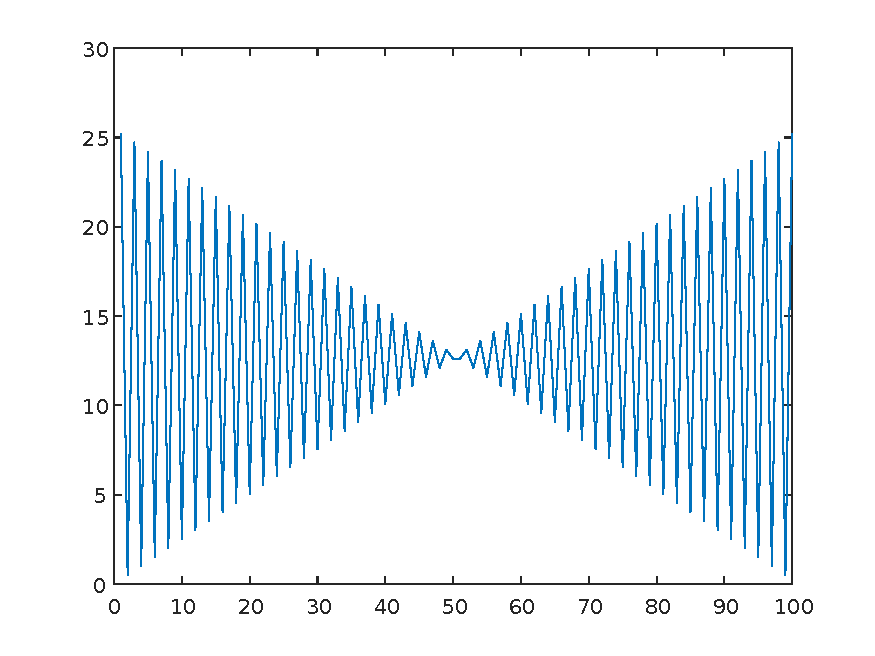
\includegraphics[]{./esercizi/imgs/graficonewtonj.pdf}
\end{center}

\section{
  Costruire una function, \textbf{lagrange.m}, avente la \underline{stessa sintassi} della function spline
  di Matlab, che implementi, in modo \underline{vettoriale}, la forma di Lagrange del polinomio interpolante una
  funzione.
  \\
  \textbf{N.B.:} il risultato dovra' avere \underline{le stesse dimensioni} del dato di ingresso; questo vale anche per gli
  esercizi a seguire.
 }

\begin{lstlisting}[style=Matlab-editor]
function s = lagrange(x, y, xq)
%s = lagrange(x, y, xq)
%Input:
%x = Vettore contenete le ascisse d'interpolazione.
%y = Vettore contenete i valori della funzione nelle ascisse d'interpolazione.
%xq = Vettore contenente le ascisse in cui vogliamo approssimare la funzione.
%Output:
%s = Valori approssimati della funzione.
%Calcola i valori approssimati della funzione, ottenuti mediante il polinomio interpolante, in forma di Lagrange, nelle ascisse xq.
  
if(length(x) ~= length(unique(x))), error("Le ascisse d'interpolazione non sono distinte tra loro." + newline + "Riprovare."),end 
if(length(x) ~= length(y)), error("Il numero delle ascisse d'interpolazione e quello dei valori della funzione non corrisponde." + newline + "Riprovare."),end
if(isempty(xq)), error("Il vettore contenente le ascisse in cui interpolare la funzione e' vuoto." + newline + "Riprovare."),end
if(size(x,2) > 1 || size(y,2) > 1 || size(xq,2) > 1),error("Non sono stati inseriti correttamente i vettori colonna." + newline + "Riprovare."),end
   
n = size(x, 1);
Lin = ones(size(xq, 1), n);
%Calcolo la produttoria Lin(x)
for i = 1 : n
    for j = 1 : n
        if (i~=j)
            Lin(:,i)=Lin(:,i).*((xq-x(j))/(x(i)-x(j)));
        end
    end
end
s = zeros(size(xq));
%Calcolo la sommatoria fi*Lin(x)
for i=1:n
    s = s+y(i).*Lin(:,i);
end
end
\end{lstlisting}

Per creare questa \textit{function} si e' andati, inizialmente, a calcolare la 
produttoria \[ Lin(x) = \prod_{j = 0, j != i}^{n} \frac{x - x_j}{x_i - x_j} \]
e successivamente la sommatoria \[ p(x) = \sum_{i = 0}^{n} f_i * L_{in}(x). \]

\section{
  Costruire una function, \textbf{newton.m}, avente la \underline{stessa sintassi} della function \textbf{spline}
  di Matlab, che implementi, in modo \underline{vettoriale}, la forma di Newton del polinomio interpolante una
  funzione.
 }
 \begin{lstlisting}[style=Matlab-editor]
function s = newton(x, y, xq)
%s = newton(x, y, xq)
%Input:
%x = Vettore colonna contenete le ascisse d'interpolazione.
%y = Vettore colonna contenete i valori della funzione nelle ascisse d'interpolazione.
%xq = Vettore contente le ascisse in cui vogliamo approssimare la funzione.
%Output:
%s = Valori approssimati della funzione.
%Calcola i valori approssimati della funzione, ottenuti attraverso il polinomio interpolante in forma di Newton nelle ascisse xq.
  
if(length(x) ~= length(unique(x))), error("Le ascisse d'interpolazione non sono distinte tra loro." + newline + "Riprovare."),end 
if(length(x) ~= length(y)), error("Il numero delle ascisse d'interpolazione e quello dei valori della funzione non corrisponde." + newline + "Riprovare."),end
if(isempty(xq)), error("Il vettore contenente le ascisse in cui interpolare la funzione e' vuoto." + newline + "Riprovare."),end
if(size(x,2) > 1 || size(y,2) > 1 || size(xq,2) > 1),error("Non sono stati inseriti correttamente i vettori colonna." + newline + "Riprovare."),end
 
diff_divise = differenze_divise(x, y);
n = length(diff_divise) - 1;
s = diff_divise(n+1) * ones(size(xq));
  
%Uso l'algoritmo di Horner per ridurre il numero di operazioni
for i=n:-1:1
    s = s.*(xq-x(i)) + diff_divise(i);  
end
return;
end
  
function diff_divise = differenze_divise(x, f)
%Calcola le differenze divise
n = size(x);
if(n ~= length(f)), error("La dimensione di x e quella di f non coincidono." + newline + "Riprovare."), end
diff_divise = f;
n = n-1;
for i = 1 : n
    for j = n + 1 : -1 : i + 1
        diff_divise(j) = (diff_divise(j) - diff_divise(j-1))/(x(j) - x(j-i));
    end
end
return;
end
\end{lstlisting}

Per creare questa \textit{function} si e' andati, inizialmente, a calcolare il
vettore delle differenze divise, implementato nella \textit{function differenze\_divise}, e
successivamente si e' andati ad utilizzare l'algoritmo di Horner, per ridurre
il numero di operazioni, per calcolare i valori del polinomio nelle ascisse \textit{xq}.


\section{
  Costruire una function, \textbf{hermite.m}, avente sintassi
  $$ yy = hermite( xi, fi, f1i, xx) $$
  che implementi, in modo \underline{vettoriale}, il polinomio interpolante di Hermite.
 }
\begin{lstlisting}[style=Matlab-editor]
function yy = hermite(xi, fi, f1i, xx)
%yy = hermite(xi, fi, f1i, xx)
%Input:
%xi = Vettore colonna contenente le ascisse d'interpolazione.
%fi = Vettore colonna contenente i valori della funzione nelle ascisse d'interpolazione.
%f1i = Vettore colonna contenente i valori della derivata prima, che assume nelle ascisse d'interpolazione.
%xx = Vettore contenente le ascisse in cui vogliamo approssimare la funzione.
%Output:
%yy = Valori approssimati della funzione con il polinomio interpolante di hermite.
%Calcola i valori approssimati della funzione, calcolati attraverso il polinomio interpolante in forma di Lagrange nelle ascisse xx.
  
if(length(xi) ~= length(unique(xi))), error("Le ascisse d'interpolazione non sono distinte tra loro." + newline + "Riprovare."),end 
if(length(xi) ~= length(fi)), error("Il numero delle ascisse d'interpolazione e quello dei valori della funzione non corrisponde." + newline + "Riprovare."),end
if(isempty(xx)), error("Il vettore xx non contiene alcuna ascissa." + newline + "Riprovare."), end  
if(length(fi) ~= length(f1i)), error("La lunghezza di fi non corrisponde a quella di f1i." + newline + "Riprovare."),end
if(size(xi,2)>1 || size(fi,2)>1 || size(f1i,2)>1), error("Non sono stati inseriti correttamente i vettori colonna." + newline + "Riprovare."),end
  
n = (length(xi));
fi(1:2:2*n-1) = fi;
fi(2:2:2*n) = f1i;
  
diff_divise = differenze_divise(xi, fi');
    
n = length(diff_divise)-1;
yy = diff_divise(n+1)*ones(size(xx));    
%Uso l'algoritmo di Horner per ridurre il numero di operazioni
for i = n:-1:1
    yy = yy.*(xx-xi(ceil(i/2)))+diff_divise(i);
end
return;
end
    
function f = differenze_divise(x, f)
%f = differenze_divise(x, f)
%Input:
%x = Vettore colonna contenente le ascisse d'interpolazione.
%f = Vettore colonna contenente i valori della funzione nelle ascisse d'interpolazione.
%Output:
%f = Differenze divise calcolate.
%Calcola le differenze divise
n = (length(f)/2)-1;
 
for i = 2*n+1:-2:3
    f(i) = (f(i)-f(i-2))/(x(ceil(i/2))-x(ceil((i-1)/2)));
end
for j = 2:2*n+1
    for i = (2*n+2):-1:j+1
        f(i) = (f(i)-f(i-1))/(x(ceil(i/2))-x(ceil((i-j)/2)));
    end
end
return;
end
\end{lstlisting}

Simile alla \textit{function} precedente, solamente che qui si sono utilizzate
anche le derivate prime della funzione che deve essere interpolata.

\section{
Costruire una function Matlab che, specificato in ingresso il grado n del polinomio
interpolante, e gli estremi dell'intervallo [a, b], calcoli le corrispondenti ascisse di Chebyshev.
}
\begin{lstlisting}[style=Matlab-editor]
function x = chebyshev(n, a, b)
%x = chebyshev(n, a, b)
%Input:
%n = Grado del polinomio
%a, b = Estremi dell'intervallo.
%Output:
%x = Ascisse di Chebyshev.
%Calcola le ascisse di Chebyshev.
if nargin < 3
    error("Il numero degli argomenti e' errato." + newline + "Riprovare.");
elseif n <= 0 || n ~= fix(n)
        error("Il grado del polinomio deve essere positivo." + newline + "Riprovare.");
elseif a >= b
        error("L'intervallo e' stato inserito in maniera non corretta." + newline + "Riprovare.");
end

x = cos(((2*(0:n) + 1)*pi)/(2*(n+1))); %Ascisse su [-1,1]
x = (a+b)/2 + (b-a)/2*x;

return;
end
\end{lstlisting}

Per creare questa \textit{function} si e' andati, inizialmente, a calcolare le ascisse
di Chebyshev nell'intervallo $ [-1, 1] $ utilizzando la seguente formula: 
\[ x_i = \cos \left( \frac{2i + 1}{2(n+1)} \pi \right) \]
e successivamente si e' andati a riportarle per il generico intervallo $ [a, b] $, 
mediante la formula:
\[ x_{n-i} = \frac{a + b}{2} + \frac{b - a}{2} * \cos \left( \frac{2i + 1}{2(n+1)} \pi \right) \]
per i che va da 0 ad \textit{n}, dove \textit{n} e' il grado del polinomio.

\section{
  Costruire una function Matlab, con sintassi
  $$ ll = lebesgue( a, b, nn, type ), $$
  che approssimi la costante di Lebesgue per l'interpolazione polinomiale sull'intervallo \textbf{[a,b]}, per
  i polinomi di grado specificato nel vettore \textbf{nn}, utilizzando ascisse equidistanti, se \textbf{type=0}, o di
  Chebyshev, se \textbf{type=1} (utilizzare 10001 punti equispaziati nell'intervallo \textbf{[a,b]} per ottenere cia-
  scuna componente di ll). Graficare i risultati ottenuti, per \textbf{nn=1:100}, utilizzando \textbf{[a,b]=[0,1]} e
  \textbf{[a,b]=[-3,7]}. Giustificare i risultati ottenuti.
}
\begin{lstlisting}[style=Matlab-editor]
function ll = lebesgue(a, b, nn, type)
%ll = lebesgue(a, b, nn, type)
%Input:
%a,b = Estremi dell'intervallo.
%nn = Vettore contenente i gradi dei polinomi.
%type = Tipologia scelta per risolvere l'esercizio.
%Output:
%ll = Approssimazione della costante di Lebesgue.
%Calcola l'approssimazione della costante di Lebesgue sull'intervallo [a, b].

if nargin < 4
    error("Il numero degli argomenti e' errato." + newline + "Riprovare.");
elseif type ~= fix(type) || type < 0 || type > 1
    error("Il valore di type non e' corretto." + newline + "Riprovare.");
elseif a >= b
    error("Intervallo errato." + newline + "Riprovare.");
end
  
x = linspace(a, b, 10001)';
ll = zeros(size(nn));

%Per ogni grado del polinomio -> Sommatoria
for i = 1 : length(nn)
    grado = nn(i);
    if type == 0
        xi = linspace(a, b, grado + 1);
    elseif type == 1
        xi = chebyshev(grado + 1, a, b);
    end

    Lin = ones(length(x), 1);
 
    for r = 1 : length(xi)
        temp = 1;
        %Produttoria 
        for j = 1 : length(xi)
            if j ~= r            
                temp = temp .* ((x - xi(j)) ./ (xi(r) - xi(j)));
            end
        end
        Lin = Lin + abs(temp);
    end
    ll(i) = max(Lin);
end
return;
end
\end{lstlisting}
\includegraphics*[scale=0.33]{./esercizi/imgs/grafico_lebesgue.pdf}
\\
Com'è possibile osservare, la costante di \textit{Lebesgue} cresce molto rapdiamente 
utilizzando ascisse d'interpolazione equidistanti tra loro, mentre questo non succede
se si utilizzano le ascisse di Chebyshev, le quali permettono una crescita piu'
lenta rispetto le prime.

\section{
  Utilizzando le function dei precedenti esercizi, graficare (in semilogy) l'andamento
  errore di interpolazione (utilizzare 10001 punti equispaziati nell'intervallo per ottenerne la stima)
  per la funzione di Runge,
  $$ f(x) = \frac{1}{1+x^2}, x\in[-5,5], $$
  utilizzando sia le ascisse equidistanti che di Chebyshev, per i polinomi interpolanti di grado \textbf{nn=2:2:100}.
  Graficare l'errore di interpolazione anche per i polinomi interpolanti di Hermite di grado \textbf{nn=3:2:99},
  sia utilizzando ascisse equidistanti che ascisse di Chebyshev, nell'intervallo considerato.
 }
 Di seguito viene riportato il grafico dell'andamento dell'errore d'interpolazione, che cambia a seconda
 della \textit{function} utilizzata e del tipo di ascisse usate.
 \\
 \includegraphics*[scale=0.80]{./esercizi/imgs/grafico_21.pdf}

\newpage
\section{
  Costruire una function, \textbf{myspline.m}, avente sintassi
  $$ yy = myspline( xi, fi, xx, type ) $$
  dove \textbf{type=0} calcola la \textit{spline} cubica interpolante naturale i punti \textbf{(xi,fi)}, e \textbf{type~=0} calcola quella
  \textit{not-a-knot} (default).
 }
\begin{lstlisting}[style=Matlab-editor]
function yy = myspline(xi, fi, xx, type)
%yy = myspline(xi, fi, xx, type)
%Input:
%xi = Valori delle ascisse.
%fi = Valori della funzione calcolati nelle ascisse.
%xx = Vettore contenente le ascisse a cui voglio approssimare la funzione.
%type = Tipologia per risolvere l'esercizio.
%Output:
%yy = Spline calcolata.
%Calcola la spline cubica interpolante naturale oppure la not-a-knot, a
%seconda del valore di type.

if nargin < 4
    error("Il numero degli argomenti e' errato." + newline + "Riprovare.");
elseif length(xi) ~= length(fi)
    error("La lunghezza dei due vettori non corrisponde." + newline + "Riprovare.");
elseif length(xi) ~= length(unique(xi))
    error("Le ascisse di interpolazione non sono distinte tra loro." + newline + "Riprovare.");
elseif size(xi, 2) > 1 || size(fi, 2) > 1
    error("Non e' stato inserito un vettore colonna correttamente." + newline + "Riprovare.")
elseif isempty(xx)
    error("La partizione assegnata e' vuota." + newline + "Riprovare.");
end

n = length(xi) - 1;
epsilon = zeros(n-1,1); %Vettore sovradiagonale
q = zeros(n-1,1); %Vettore sottodiagonale

for i = 2 : n
    hi = (xi(i) - xi(i-1));
    hi1 = (xi(i+1) - xi(i));
    q(i-1) = hi / (hi + hi1);
    epsilon(i-1) = hi1 / (hi + hi1);
end

diff_div = diff_div_spline(xi, fi); %Calcolo le differenze divise

a = 2*ones(n-1,1);
if type == 0
    m = tridia(a, epsilon, q, diff_div * 6);
    m = [0; m; 0];
else
    diff_div = diff_div * 6;

    a(1) = 2 - q(1);
    epsilon(1) = epsilon(1) - q(1);
    diff_div_1 = diff_div(1);
    diff_div(1) = (1 - q(1)) * diff_div(1);
    q(1) = 0;

    a(n-1) = 2 - epsilon(n-1);
    q(n-1) = q(n-1) - epsilon(n-1);
    diff_div_n = diff_div(n-1);
    diff_div(n-1) = (1 - epsilon(n-1)) * diff_div(n-1);
    epsilon(n-1) = 0;

    m = tridia(a, epsilon, q, diff_div);

    m0 = diff_div_1 - m(1) - m(2);
    mn = diff_div_n - m(n-1) - m(n-2);
    m = [m0; m; mn];
end

yy = calcola_punti(xi, fi, m, xx);
return;
end

function diff_div = diff_div_spline(xi, fi)
%diff_div = diffdivspline(xi, fi)
%Input:
%xi = Valori delle ascisse.
%fi = Valori della funzione calcolati nelle ascisse.
%Output:
%diff_div = Differenze divise calcolate.
%Calcola le differenze divise per la spline

n = size(xi);
diff_div = fi;
n = n-1;
for j = 1 : 2
    for i = n+1 : -1 : j+1
        diff_div(i) = (diff_div(i) - diff_div(i-1))/(xi(i) - xi(i-j));
    end
end
diff_div = diff_div(3:n+1);
return;
end

function x = tridia(a, b, c, g)
%x = tridia(a, b, c, g)
%Input:
%a = Vettore diagonale principale.
%b = Vettore sovradiagonale.
%c = Vettore sottodiagonale.
%g = Vettore dei termini noti.
%Output:
%x = Vettore soluzione.
%Risoluzione di un sistema tridiagonale.

n = length(g);
x = g;
for i = 1 : n-1
    b(i) = b(i)/a(i);
    a(i+1) = a(i+1) - b(i)*c(i);
    x(i+1) = x(i+1) - b(i)*x(i);
end

x(n) = x(n)/a(n);
for i = n-1 : -1 : 1
    x(i) = (x(i) - c(i)*x(i+1))/a(i);
end
return;
end

function yy = calcola_punti(xi, fi, m, xx)
%yy = calcola_punti(xi, fi, m, xx)
%Input:
%xi = Valori delle ascisse.
%fi = Valori della funzione calcolati nelle ascisse.
%m = Matrice dei coefficienti.
%xx = Partizione assegnata.
%Output:
%yy = Valori della spline.
%Calcola i valori della spline nei punti definiti in xx.

yy = zeros(length(xx), 1);

for j = 1 : length(xx)
    for i = 2 : length(xi) 
        if((xx(j) >= xi(i-1) && xx(j) <= xi(i)) || xx(j) < xi(1))
            hi = xi(i)-xi(i-1);
            ri = fi(i-1)-hi^2/6*m(i-1);
            qi = (fi(i)-fi(i-1))/hi-hi/6*(m(i)-m(i-1));
            yy(j) =((xx(j)-xi(i-1))^3*m(i)+(xi(i)-xx(j))^3*m(i-1))/(6*hi)+qi*(xx(j)-xi(i-1))+ri;
            break
        end
    end
end
return;
end
\end{lstlisting}

\section{
Graficare, utilizzando il formato semilogy, l'errore di approssimazione utilizzando le
\textit{spline} interpolanti naturale e \textit{not-a-knot} per approssimare la funzione di Runge sull'intervallo $ [-5,5] $,
utilizzando una partizione $ \delta = {-5 = x_0 < \cdots < x_n = 5} $, con ascisse equidistanti e \textbf{n=4:4:400}.
\\
Utilizzare 10001 punti equispaziati nell'intervallo $ [-5,5] $ per ottenere la stima dell'errore.
}
Di seguito viene riportato il grafico dell'andamento dell'errore di approssimazione, utilizzando
le \textit{spline} interpolanti naturale e \textit{not-a-knot}, per approssimare la funzione di 
Runge nell'intervallo desiderato.
\\
\includegraphics*[scale=0.80]{./esercizi/imgs/grafico_23.pdf}


\section{
  E' noto che un fenomeno fisico evolve come $ y = x^n$, con \textit{n} incognito. Il file \textbf{data.mat},
  reperibile a:
  $$ https://drive.google.com/file/d/14u2Pjnl_BZN1GWEFCZd0tqKCObGGI-M5 $$
  $$ /view?usp=share_link $$
  contiene 1000 coppie di dati $ (x_i, y_i) $, in cui la seconda componente `e affetta da un errore con di-
  stribuzione Gaussiana a media nulla e varianza "piccola". Utilizzando un opportuno polinomio
  di approssimazione ai minimi quadrati, stimare il grado \textit{n}. Argomentare il procedimento seguito,
  graficando la norma del residuo rispetto a valori crescenti di n. `E richiesto il codice Matlab dell'al-
  goritmo che avrete implementato (potete utilizzare, se lo ritenete opportuno, la function \textbf{polyfit}
  di Matlab).
 }
Di seguito viene riportato lo script usato per andare a stimare il grado \textit{n}:
\\
\begin{lstlisting}[style=Matlab-editor]
load("data.mat");
format lonG;
x = data(:, 1);
y = data(:, 2);
errori = zeros(10, 1);
for i = 1 : 10
  p = polyfit(x, y, i);
  y_tilde = polyval(p, x);
  errori(i) = norm(x.^i - y_tilde);
end

[errore, grado] = min(errori);
disp(errore);
disp(grado);

plot(1:10, errori);
xlabel("Grado del polinomio");
ylabel("Norma del residuo");
\end{lstlisting}

Per la realizzazione di questo Script si e' andati inizialmente a caricare i dati forniti nel file 
\textit{data.mat} ed inizializzare il vettore contenente gli errori.
Dopodichè, siamo andati a calcolarci i coefficienti del polinomio mediante la funzione \textit{polyfit} di
Matlab e a valutare il valore del polinomio.
Successivamente, dato che sapevamo che il fenomeno sarebbe cresciuto come \textit{y = $ x^n $}, abbiamo
calcolato l'errore commesso.
Infine, abbiamo preso il grado minimo \textit{n} mediante la funzione \textit{min} fornita da Matlab e abbiamo
creato il grafico, il quale viene riportato di seguito.
\\
\includegraphics*[scale=0.80]{./esercizi/imgs/grafico_24.pdf}


\section{
  Costruire una function Matlab che, dato in input \textit{n}, restituisca i pesi della qua-
  dratura della formula di Newton-Cotes di grado \textit{n}. Tabulare, quindi, i pesi delle formule di grado
  1, 2,. . . , 7 e 9 (come \underline{numeri razionali}).
 }
\begin{lstlisting}[style=Matlab-editor]
function coefficienti = coefficienti_newton_cotes(n)
%coefficienti = coefficienti_newton_cotes(n)
%Input:
%n = Grado della formula di Newton-Cotes.
%Output:
%coefficienti = Coefficienti della formula di Newton-Cotes.
%Restituisce i pesi della quadratura della formula di Newton-Cotes di grado n.

if n <= 0 || n == 8 || n > 9, error("Il grado del polinomio deve essere compreso tra 1 e 7 oppure uguale a 9." + newline +  "Riprovare."), end

coefficienti = zeros(1, n+1);

for i = 0 : n
    k = [0:i-1 i+1:n];
    denominatore = prod(i-k);
    p = poly(k);
    p = [p ./ ((n+1):-1:1) 0];
    numeratore = polyval(p, n);
    coefficienti(i+1) = numeratore/denominatore;
end

return;
end
\end{lstlisting}

Di seguito viene riportata la tabella contente i pesi calcolati, per ogni grado della formula.
\\
\begin{center}
  \begin{spacing}{1.5}
  \begin{longtable}{ |p{0.2cm}|p{8cm}| }
    \hline
    \multicolumn{2}{|c|}{ \textbf{Dati - Tabella di confronto}} \\
    \hline
    \textbf{n}     & \textbf{Pesi} \\
    \hline
    1 & $ \frac{1}{2}, \frac{1}{2} $ \\
    2 & $ \frac{1}{3}, \frac{4}{3}, \frac{1}{3} $ \\
    3 & $ \frac{3}{8}, \frac{9}{8}, \frac{9}{8}, \frac{3}{8} $ \\
    4 & $ \frac{14}{45}, \frac{64}{45}, \frac{8}{15}, \frac{64}{45}, \frac{14}{45} $ \\
    5 & $ \frac{95}{288}, \frac{125}{96}, \frac{125}{144}, \frac{125}{144}, \frac{125}{96}, \frac{95}{288} $ \\
    6 & $ \frac{41}{140}, \frac{54}{35}, \frac{27}{140}, \frac{68}{35}, \frac{27}{140}, \frac{54}{35}, \frac{41}{140}, $ \\
    7 & $ \frac{1073}{3527}, \frac{810}{559}, \frac{343}{640}, \frac{649}{536}, \frac{649}{536}, \frac{343}{640}, \frac{810}{559}, \frac{1073}{3527} $ \\
    9 & $ \frac{130}{453}, \frac{1374}{869}, \frac{243}{2240}, \frac{5287}{2721}, \frac{704}{1213}, \frac{704}{1213}, \frac{5594}{2879}, \frac{243}{2240}, \frac{1374}{869}, \frac{130}{453} $ \\
    \hline
  \end{longtable}
\end{spacing}
\end{center}

\newpage
\section{
  Scrivere una function Matlab,
  $$ [If,err] = composita( fun, a, b, k, n ) $$
  che implementi la formula composita di Newton-Cotes di grado \textbf{k} su \textbf{n+1} ascisse equidistanti, con \textbf{n}
  multiplo pari di \textbf{k}, in cui:
  \\
  \textbullet \textbf{fun} e' la funzione integranda (che accetta input vettoriali);
  \\
  \textbullet \textbf{[a,b]} e' l'intervallo di integrazione;
  \\
  \textbullet \textbf{k, n} come su descritti;
  \\
  \textbullet \textbf{If} e' l'approssimazione dell'integrale ottenuta;
  \\
  \textbullet \textbf{err} e' la stima dell'errore di quadratura.
 }
\begin{lstlisting}[style=Matlab-editor]
function [If, err] = composita(fun, a, b, k, n)
%[If, err] = composita(fun, a, b, k, n)
%Input:
%fun = Identificatore function della funzione integranda
%a,b = Estremi dell'intervallo di integrazione.
%k = Grado del polinomio
%n = Numero delle ascisse.
%Output:
%If = Approssimazione dell'integrale ottenuta.
%err = Stima dell'errore di quadratura.
%Calcolo della formula composita di Newton-Cotes di grado k u n+1 ascisse
%equidistanti, con n multiplo pari di k.

if a >= b, error("L'intervallo e' stato inserito in maniera non corretta." + newline + "Riprovare."), end
if k <= 0, error("Il grado del polinomio deve essere positivo." + newline + "Riprovare."), end
if n <= 0, error("Il numero delle ascisse non e' corretto."+ newline + "Riprovare."), end
if mod(n, 2) ~= 0, error("Il numero delle ascisse non e' un multiplo pari di k." + newline + "Riprovare."), end

mu = 1;
if mod(n, 2) ~= 0
  mu = 2;
end

coefficienti = coefficienti_newton_cotes(k);
h = (b-a)/n;

If = 0;
I1 = 0;
for i = 0:n-1
  x = linspace(a + i*h, a + (i+1)*h, k+1);
  fx = feval(fun, x);
  If = If + (h/k)*sum(fx.*coefficienti);
  if mod(i,2) == 0
      I1 = I1 + (h/(2*k))*sum(fx.*coefficienti);
  end
end

err = abs(If-I1)/(2^(k+mu)-1);

return;
end
\end{lstlisting}

\section{
Utilizzare la function \textbf{composita} per ottenere l'approssimazione dell'integrale
$$
  \int_{0}^{1}
  (\sum_{i=1}^{5} i \cos 2 \pi ix - e^i \sin 2(\pi i + 0.1)x)
  \, dx
$$
con le formule composite di Newton-Cotes di grado \textbf{k=1,2,3,6}. Per tutte, utilizzare \textbf{n=12}.
}

Di seguito e' riportata la tabella dei dati, riguardanti le approssimazioni di \textbf{If}
e le stime degli errori, per i valori di \textbf{k} forniti dall'esercizio.
\\
\begin{center}
  \begin{tabular}{ |p{3.7cm}|p{3cm}|p{0.5cm}| }
    \hline
    \multicolumn{3}{|c|}{ \textbf{Tabella dei dati}} \\
    \hline
    \textbf{If} & \textbf{Errore} & \textbf{k}      \\
    \hline
    -0.0925980476169039 & 0.184019370137441 & 1 \\
    -0.179803240495078  & 0.188624769819435 & 2 \\
    -0.17847075804203  & 0.0871853736641679 & 3 \\
    -0.17744651109262 & 0.0102213795366299 & 6 \\
    \hline
  \end{tabular}
\end{center}

\section{
  Implementare la formula composita adattativa di Simpson.
 }
\begin{lstlisting}[style=Matlab-editor]
function [I2, nvalfunz] = adapsim(a, b, f, tol, fa, f1, fb)
%[I2, nvalfunz] = adapsim(a, b, f, tol, fa, f1, fb)
%Input:
%a,b = Estremi dell'intervallo.
%f = Funzione integranda.
%tol = Tolleranza massima.
%fa = Funzione calcolata nell'estremo a.
%f1 = Funzione calcolata nel punto medio.
%fb = Funzione calcolata nell'estremo b.
%Output:
%I2 = Approssimazione calcolata.
%nvalfunz = Numero di valutazioni funzionali.
%Calcola l'approssimazione dell'integrale mediante la formula adattiva Simpson.
  
if tol <= 0, error("La tolleranza deve essere positiva." + newline + "Riprovare."), end
if a >= b, error("L'intervallo e' stato inserito in maniera non corretta." + newline + "Riprovare."), end
  
x1 = (a+b)/2;
nvalfunz = 0;
if nargin <= 4
    fa = feval(f, a);
    f1 = feval(f, x1);
    fb = feval(f, b);
    nvalfunz = nvalfunz + 3;
end
  
h = (b-a)/6;
  
x2 = (a+x1)/2;
x3 = (x1+b)/2;
  
f2 = feval(f, x2);
f3 = feval(f, x3);
nvalfunz = nvalfunz + 2;
  
I1 = h * (fa + 4*f1 + fb);
I2 = (h/2) * (fa + 4*f2 + 2*f1 + 4*f3 + fb);
err = abs(I2 - I1)/15;
  
if err > tol
    [I2s, nvalfunzs] = adapsim(a, x1, f, tol/2, fa, f2, f1);
    [I2d, nvalfunzd] = adapsim(x1, b, f, tol/2, f1, f3, fb);
    I2 = I2s + I2d;
    nvalfunz = nvalfunz + nvalfunzs + nvalfunzd;
end
return;
end
\end{lstlisting}

\section{
  Implementare la formula composita adattativa di Newton-Cotes di grado \textbf{k=4}.
 }
\begin{lstlisting}[style=Matlab-editor]
function [I2, nvalfunz] = composita_adattiva_newton_cotes_4(a, b, f, tol, fa, fm, f2, f3, fb)
%[I2, nvalfunz] = composita_adattiva_newton_cotes_4(a, b, f, tol, fa, fm, f2, f3, fb)
%Input:
%a,b = Estremi dell'intervallo.
%f = Funzione integranda.
%tol = Tolleranza massima.
%fa = Funzione calcolata nell'estremo a.
%fm = Funzione calcolata nel punto medio.
%f2 = Funzione calcolata nel punto compreso tra l'estremo sinistro ed il punto medio. 
%f3 = Funzione calcolata nel punto compreso tra il punto medio e l'estremo
%destro
%fb = Funzione calcolata nell'estremo b.
%Output:
%I2 = Approssimazione calcolata.
%nvalfunz = Numero di valutazioni funzionali.
%Calcola l'approssimazione dell'integrale mediante la formula adattiva di Newton-Cotes di grado k = 4.

if tol <= 0, error("La tolleranza deve essere positiva." + newline + "Riprovare."), end
if a >= b, error("L'intervallo e' stato inserito in maniera non corretta." + newline + "Riprovare."), end

xm = (a+b)/2;
x2 = (a+xm)/2;
x3 = (xm+b)/2;

nvalfunz = 0;
if nargin <= 4
    fa = feval(f, a);
    fb = feval(f, b);
    fm = feval(f, xm);
    f2 = feval(f, x2);
    f3 = feval(f, x3);
    nvalfunz = nvalfunz + 5;
end

h = (b-a)/90;

I1 = h * (7*fa + 32*f2 + 12*fm + 32*f3 + 7*fb);

x4 = (a + x2)/2;
x5 = (x2 + xm)/2;
x6 = (xm + x3)/2;
x7 = (x3 + b)/2;

f4 = feval(f, x4);
f5 = feval(f, x5);
f6 = feval(f, x6);
f7 = feval(f, x7);
nvalfunz = nvalfunz + 4;

I2 = h/2 * (7*fa + 32*f4 + 12*f2 + 32*f5 + 14*fm + 32*f6 + 12*f3 + 32*f7 + 7*fb);

err = abs(I2-I1)/63;

if err > tol
    [I2s, nvalfunzs] = composita_adattiva_newton_cotes_4(a, xm, f, tol/2, fa, f2, f4, f5, fm);
    [I2d, nvalfunzd] = composita_adattiva_newton_cotes_4(xm, b, f, tol/2, fm, f3, f6, f7, fb);
    I2 = I2s + I2d; 
    nvalfunz = nvalfunz + nvalfunzs + nvalfunzd;
end
return;
end
\end{lstlisting}

\section{
  Confrontare le formule adattative degli ultimi due esercizi, tabulando il numero
  di valutazioni funzionali effettuate, rispetto alla tolleranza \textbf{tol = 1e-2, 1e-3, ..., 1e-9}, per
  ottenere l'approssimazione dell'integrale
  $$
    \int_{10^{-5}}^{1}
    x^{-1} \cos(\log x^{-1})
    \, dx \equiv \sin \log 10^5.
  $$
  Costruire un'altra tabella, in cui si tabula l'errore vero (essendo l'integrale noto, in questo caso)
  rispetto a \textbf{tol}.
 }
 Di seguito viene riportata la tabella di confronto dei dati, 
 con l'approssimazione dell'integrale ed il relativo numero di valutazioni funzionali, per ogni tolleranza richiesta. 

 \begin{center}
  \setlength\tabcolsep{2pt}
  \begin{tabular}{|p{3.6cm} | p{1cm} | p{3.6cm} | p{1cm} | p{1cm}|}
    \hline
    \multicolumn{5}{|c|}{\textbf{Dati - Tabella di confronto}}  \\                                                                                                                                 
    \hline
    \multicolumn{2}{|c|}{\textbf{Simpson}} & \multicolumn{2}{|c|}{\textbf{Newton-Cotes}} & \multicolumn{1}{c|}{\textbf{//}} \\                                                                           
    \hline
    \multicolumn{1}{|c|}{\textbf{I2}} & \multicolumn{1}{|c|}{\textbf{Num. val. funz.}} & \multicolumn{1}{|c|}{\textbf{I2}} &
     \multicolumn{1}{|c|}{\textbf{Num. val. funz.}}  & \multicolumn{1}{|c|}{\textbf{Tol.}} \\
    \hline
    0.000293528025694378 & 201 & 2.30517976296252e-06 & 153 & 1e-2 \\
    0.000457223923411743 & 333 & 1.06536073019026e-06 & 193 & 1e-3 \\
    2.63547596144331e-05 & 605 & 9.8526042879854e-10 & 257 & 1e-4 \\
    2.34481367566985e-06 & 1061 & 3.10416783644296e-06 & 369 & 1e-5 \\
    3.0076262513834e-07 & 1869 & 3.6973281103414e-08 & 553 & 1e-6 \\
    3.65647581102024e-08 & 3277 & 2.28150851544484e-08 & 793 & 1e-7 \\
    3.21109816514564e-09 & 5921 & 2.13358375411588e-09 & 1177 & 1e-8 \\
    3.09839487400154e-10 & 10589 & 1.49663170745384e-10 & 1753 & 1e-9 \\
    \hline
\end{tabular}
\end{center}
\end{document}